\documentclass{../source/Paper}

%关键信息输入
\major{专业}
\name{姓名}
\articletitle{论文标题}
\stuid{1008611}
\college{学院}
\date{\today}
\course{课程名称}
\instructor{}
%摘要
\Abstract{大不自多,海纳江河。惟学无际,际于天地。形上谓道兮,形下谓器。礼主别异兮,乐主和同。知其不二兮,尔听斯聪。国有成均,在浙之滨。昔言求是,实启尔求真。习坎示教,始见经纶。无曰已是,无曰遂真。靡革匪因,靡故匪新。何以新之,开物前民。嗟尔髦士,尚其有闻。念哉典学,思睿观通。有文,有质,有农,有工。兼总条贯,知至知终。成章乃达,若金之在熔。尚亨于野,无吝于宗。树我邦国,天下来同。}
%关键词
\Keyword{有文、有质、有农、有工、ZJU}


\begin{document}
    \makeheader

    \section{测试文字一}
        \subsection{测试文字1}
        \subsubsection{测试文字1.1}
        大不自多,海纳江河。惟学无际,际于天地。形上谓道兮,形下谓器。礼主别异兮,乐主和同。知其不二兮,尔听斯聪。\par
        国有成均,在浙之滨。昔言求是,实启尔求真。习坎示教,始见经纶。无曰已是,无曰遂真。靡革匪因,靡故匪新。何以新之,开物前民。嗟尔髦士,尚其有闻。\par
        念哉典学,思睿观通。有文,有质,有农,有工。兼总条贯,知至知终。成章乃达,若金之在熔。尚亨于野,无吝于宗。树我邦国,天下来同。\Footnote{脚注1}(此处为了使脚注字体为楷体用了新的命令\textbackslash Footnote)
        \subsection{测试文字2}
        多图插入(图片引用可以不用输入后缀)
        \begin{figure}[htbp]
            \centering
            \begin{minipage}[t]{0.48\textwidth}
                \centering
                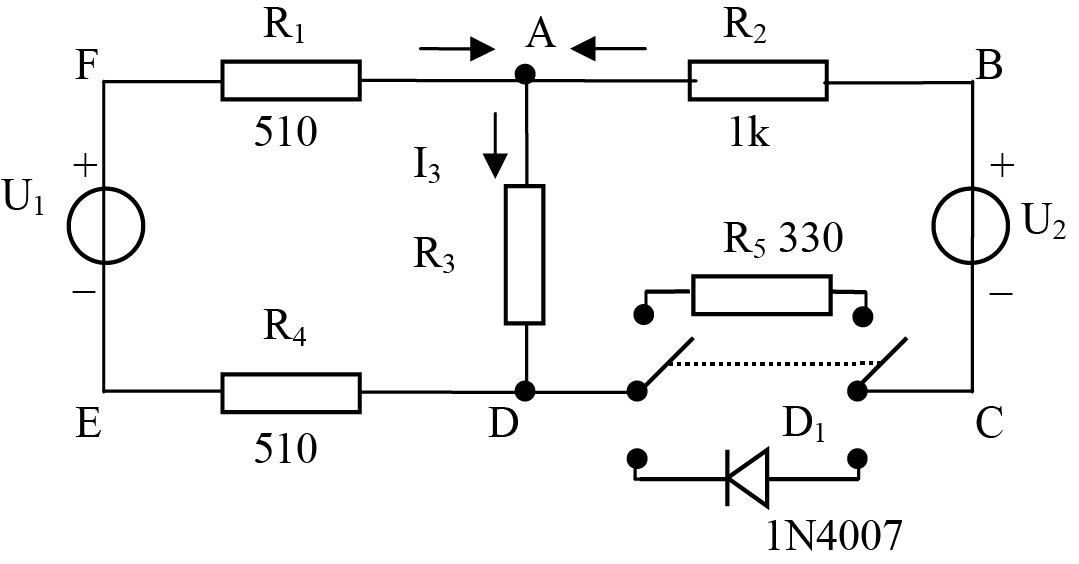
\includegraphics[width=6cm]{pic2}
                \caption{测试图片}
            \end{minipage}
            \begin{minipage}[t]{0.48\textwidth}
                \centering
                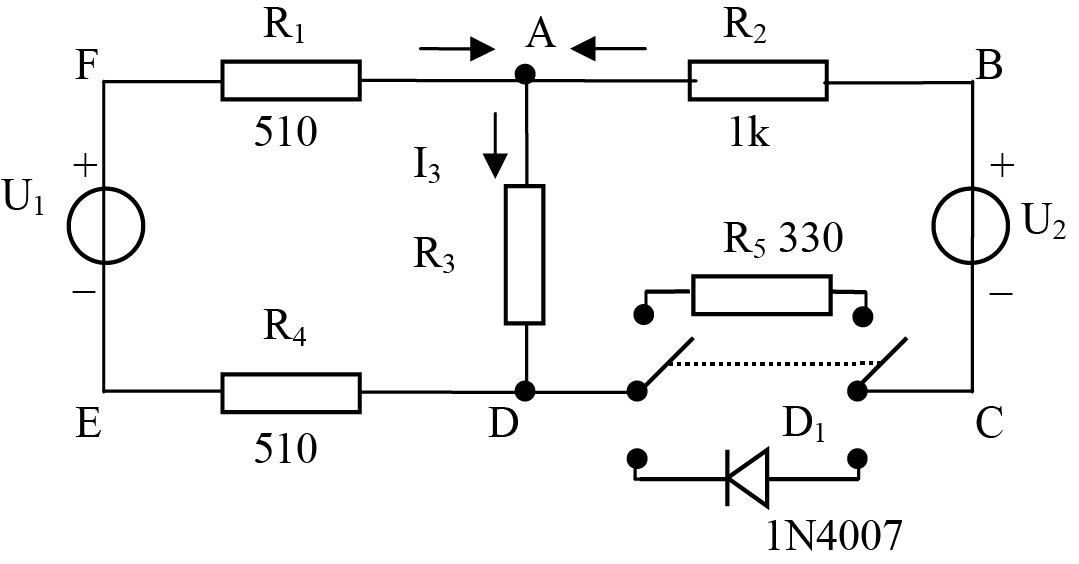
\includegraphics[width=6cm]{pic2}
                \caption{测试图片}
            \end{minipage}
        \end{figure}
    \section{测试文字二}
        大不自多,海纳江河。惟学无际,际于天地。形上谓道兮,形下谓器。礼主别异兮,乐主和同。知其不二兮,尔听斯聪。国有成均,在浙之滨。昔言求是,实启尔求真。习坎示教,始见经纶。无曰已是,无曰遂真。靡革匪因,靡故匪新。何以新之,开物前民。嗟尔髦士,尚其有闻。念哉典学,思睿观通。有文,有质,有农,有工。兼总条贯,知至知终。成章乃达,若金之在熔。尚亨于野,无吝于宗。树我邦国,天下来同。
        大不自多,海纳江河。惟学无际,际于天地。形上谓道兮,形下谓器。礼主别异兮,乐主和同。知其不二兮,尔听斯聪。\Footnote{脚注3} \par
        代码块测试:
        \begin{lstlisting}[name = 数据选择器代码]
            module mux_2to1(
                out, in0, in1, addr
            );
                parameter n = 4;        // 对n赋值为4,因为设计要求为4位
                input [n-1:0] in0, in1; // 输入4位待选择数据
                input addr;             // 输入控制信号
                output reg [n-1:0] out; // 输出4位的选择结果
            
                always @(*) begin       
                    if (addr) begin     // 如果addr = 1,输出in1
                        out = in1;
                    end
                    else begin          // 如果addr = 0,输出in2
                        out = in0;
                    end
                end
            endmodule
        \end{lstlisting}
        公式测试:
        $$\sqrt{x} + \sqrt{x^{2}+\sqrt{y}} = \sqrt[3]{k_{i}} - \frac{x}{m}$$
        
\end{document}